\documentclass{beamer}

\input{headers.tex}
\input{creative_commons/cc_beamer}

% define document details
\title[]{Best Practices}
\author{Nicola Chiapolini}
\institute{Physik-Institut\\
University of Zurich}
\date{\today}
\subject{Python School}

\begin{document}

\begin{frame}
    \titlepage
    \begin{center}
    \tiny{Based on talk by Valentin Haenel}
    \hspace{1em}
    \tiny\url{https://github.com/esc/best-practices-talk}
    \begin{tabular}[t]{lr}
        \mbox{\href{https://creativecommons.org/licenses/by-sa/3.0/}
          {\CcGroupBySa{0.35}{0.95ex}}}
        &
        \parbox[b]{8cm}{{\tiny
            \href{https://creativecommons.org/licenses/by-sa/3.0/}
            {\CcNote{\CcLongnameBySa}}}} \\
    \end{tabular}
\end{center}
\end{frame}




\section{Introduction}
\sectiontitle

\begin{frame}
 \frametitle{Introduction}

\begin{itemize}
 \item We write code regularly 
 \item We have not been formally trained
\end{itemize}

\begin{block}{Best Practices}
\begin{itemize}
 \item evolved from experience
 \item increase productivity 
 \item decrease stress
 \item still evolve with tools and languages
\end{itemize}
\end{block}

\begin{block}{Development Methodologies}
\begin{itemize}
 \item e.g. Agile Programming or Test Driven Development
 \item lots of buzzwords
 \item still many helpful ideas
\end{itemize}
\end{block}

 
\end{frame}

% -------------------------------------

\begin{frame}<1>[label=outline]
 \frametitle{Outline}

\only<1>{\tableofcontents}
\only<2->{\tableofcontents[currentsection,currentsubsection]}
  
\end{frame}

% -------------------------------------

\section{Style and Documentation}
\againframe<2>{outline}

% -------------------------------------

\begin{frame}
 \frametitle{Coding Style}

\begin{itemize}
  \item readability counts
  \item explicit is better than implicit
\end{itemize}

\begin{itemize}
  \item give variables \emph{intention revealing} names
\begin{itemize}
  \item For example: \textcolor{blue}{\texttt{numbers}} instead of \textcolor{blue}{\texttt{n}}
  \item For example: \textcolor{blue}{\texttt{numbers}} instead of \textcolor{blue}{\texttt{list\_of\_float\_numbers}}
  \item See also: \href{http://objectmentor.com/resources/articles/naming.htm}{Ottingers Rules for Naming}
\end{itemize}
\end{itemize}

\vspace{0.5cm}

\begin{example}
\pyfile{code/my_product.py}
\end{example}

\end{frame}

% -------------------------------------

\begin{frame}
 \frametitle{Formatting Code}

\begin{itemize}
  \item use coding conventions
  \item conventions specify:
\begin{itemize}
  \item variable naming
  \item indentation
  \item import
  \item maximum line length
  \item blank lines, whitespace, comments
\end{itemize}
  \item e.g: \href{http://www.python.org/dev/peps/pep-0008/}{PEP-8}
  \item OR use a consistent style (especially when collaborating)
\end{itemize}

\begin{block}{Tools}
\begin{itemize}
  \item \href{http://www.pylint.org/}{pylint}
  \item \href{https://pypi.python.org/pypi/pep8}{pep8}
  \item \href{http://pypi.python.org/pypi/flake8/}{flake8} %(combination of \texttt{pep8} and \texttt{pyflakes})
\end{itemize}
\end{block}

\end{frame}

% -------------------------------------

\begin{frame}
 \frametitle{Documenting Code: Docstrings}

\begin{example}
  \pyfile{code/my_product_minidoc.py}
\end{example}

\begin{itemize}
  \item at least a single line 
  \item also for yourself
  \item is on-line help too
\end{itemize}

\begin{itemize}
  \item Document arguments and return objects, including types
  \item For complex algorithms, document every line,\\ and include equations in docstring
  \item Use the \href{https://github.com/numpy/numpy/blob/master/doc/HOWTO_DOCUMENT.rst.txt}{numpy docstring conventions}
\end{itemize}
\end{frame}

% -------------------------------------

\begin{frame}
 \frametitle{Example Docstring}
\pyfile{code/my_product_docstring.py}
\end{frame}

% -------------------------------------

\begin{frame}
 \frametitle{Documenting Code}

\begin{columns}[T]
\column{0.5\textwidth}
\begin{itemize}
  \item tools generate website\\ from docstrings
\begin{itemize}
  \item \href{http://docs.python.org/library/pydoc.html}{pydoc}
  \item \href{http://epydoc.sourceforge.net/}{epydoc}
  \item \href{http://sphinx.pocoo.org/}{sphinx}
\end{itemize}
\end{itemize}

\begin{itemize}
  \item when project gets bigger
\begin{itemize}
  \item how-to 
  \item FAQ
  \item quick-start
\end{itemize}
\end{itemize}

\column{0.5\textwidth}
\includegraphics[width=1\textwidth]{images/sphinxdoc.png}

\end{columns}
 
\end{frame}

% -------------------------------------

\section{Special Python Statements}
\againframe<3>{outline}

% -------------------------------------

\begin{frame}[containsverbatim]
\frametitle{\texttt{import}}
  
\begin{itemize}
  \item Don't use the \emph{star import}: \texttt{from module import *}
\begin{itemize}
  \item hard to read
  \item modules may overwrite each other
  \item Where does this function come from?
  \item will import \emph{everything} in a module
  \item ...unless you have a very good reason: e.g. \texttt{pylab}, interactive
\end{itemize}
\end{itemize}

\begin{itemize}
  \item Put all imports at the beginning of the file...
  \item ...unless you have a very good reason
\end{itemize}

\begin{example}
\begin{pycode}
import my_product as mp
mp.my_product([1,2,3])
\end{pycode}

\begin{pycode}
from my_product import my_product
my_product([1,2,3])
\end{pycode}
\end{example}

\end{frame}

% -------------------------------------

\begin{frame}
 \frametitle{Exceptions}
  
\begin{itemize}
  \item use \texttt{try except} and \texttt{raise}
  \item often better then \texttt{if} (e.g. \texttt{IndexError})
\end{itemize}

\begin{example}
\pyfile{code/my_product_try.py}
\end{example}

\begin{itemize}
  \item don't use \emph{special} return values: \\
 \texttt{1}, \texttt{0}, \texttt{False}, \texttt{None}
  \item Fail early, fail often
  \item use \href{http://docs.python.org/library/exceptions.html}{built-in Exceptions}
\end{itemize}

  
\end{frame}

% -------------------------------------

\section{KIS(S) \& DRY}
\againframe<4>{outline}

% -------------------------------------

\begin{frame}
 \frametitle{Keep it Simple (Stupid) -- KIS(S) Principle}
\centering

\alert<2>{\LARGE Keep it Simple}
  
\end{frame}

% -------------------------------------

\begin{frame}
 \frametitle{Don't Repeat Yourself (DRY)}

\begin{itemize}
 \item No cupy \& paste!
\end{itemize}

\begin{itemize}
  \item Not just lines code, but knowledge of all sorts
  \item Do not express the same piece of knowledge in two places...
  \item ...or you will have to update it everywhere
\end{itemize}

\begin{itemize}
  \item It is not a question of \emph{if} this may fail, but \emph{when}
\end{itemize}
\end{frame}

% -------------------------------------

\begin{frame}[fragile]
 \frametitle{Don't Repeat Yourself (DRY): Types}
\begin{example}
\begin{itemize}
  \item Version number in source code, website, readme, package filename
  \item Copy-and-paste a snippet, instead of refactoring it into a function
  \item Repeated implementation of utility methods 
  \begin{itemize}
   \item because you don't remember
   \item because you don't know the libraries\begin{pycode}
numpy.prod([1,2,3])
\end{pycode}
   \item \alert<2>{because developers don't talk to each other}
  \end{itemize}
\end{itemize}
\end{example}
  
\begin{itemize}
  \item If you detect duplication: refactor mercilessly!
\end{itemize}

\end{frame}

% -------------------------------------

\section{Refactoring}
\againframe<5>{outline}

% -------------------------------------

\begin{frame}
 \frametitle{Refactoring}
 
\begin{itemize}
  \item re-organise your code without changing its function
\end{itemize}

\begin{itemize}
  \item rethink earlier design decisions
  \item break large code blocks apart
  \item rename and restructure code
\end{itemize}

\begin{itemize}
  \item will improve the readability and modularity
  \item will usually reduce the lines of code
\end{itemize}

\end{frame}

% -------------------------------------

\begin{frame}
 \frametitle{Common Refactoring Operations}

\begin{itemize}
  \item Rename class/method/module/package/function
  \item Move class/method/module/package/function
  \item Encapsulate code in method/function
  \item Change method/function signature
  \item Organise imports (remove unused and sort)
\end{itemize}

\begin{itemize}
  \item Always refactor one step at a time, and ensure code still works
\begin{itemize}
\item version control
\item unit tests
\end{itemize}
\end{itemize}
  
\end{frame}

% -------------------------------------

\begin{frame}
 \frametitle{Refactoring Example}

\begin{columns}[T]
\column{0.01\textwidth}
\vspace*{5cm}

\column{0.99\textwidth}
\only<1>{\pyfile{code/my_product_refactor.py}}
\only<2>{\pyfile{code/my_product_refactored-1.py}}
\only<3>{\pyfile{code/my_product_refactored-2.py}}
\only<4>{\pyfile{code/my_product_refactored-3.py}}

\end{columns}

\begin{itemize}
 \item<2> split into functions
 \item<3-> use libraries/built-ins
 \item<4-> fix bug
\end{itemize}


\end{frame}

% -------------------------------------

\section{Development Methodologies}
\againframe<6>{outline}

% -------------------------------------

\begin{frame}
 \frametitle{What is a Development Methodology?}

\begin{block}{Consists of:}
\begin{itemize}
  \item attitude, style and approach towards development
  \item tools and models to support approach
\end{itemize}
\end{block}

\begin{block}{Help answer questions like:}
\begin{itemize}
  \item How far ahead should I plan?
  \item What should I prioritise?
  \item When do I write tests and documentation?
\end{itemize}
\end{block}

\vspace*{5mm}
\centering
\alert<2>{\large Right methodology depends on scenario.}
 
\end{frame}

% -------------------------------------

\begin{frame}
 \frametitle{The Waterfall Model, Royce 1970}
  
\begin{figure}[ht]
  \includegraphics[height=0.55\textheight]{images/waterfall.pdf}
\end{figure}

\begin{itemize}
  \item sequential 
  \item from manufacturing and construction
\end{itemize}
  
\end{frame}

% -------------------------------------

\begin{frame}
 \frametitle{Agile Methods (late 90's)}

\begin{itemize}
  \item minimal planning, small development iterations
  \item design/implement/test on a modular level
  \item frequent input from team/customer/boss/professor
  \item very adaptive, since nothing is set in stone
\end{itemize}

\begin{figure}
    \includegraphics[height=0.45\textheight]{images/agile.pdf}
\end{figure}

\end{frame}

% -------------------------------------

\begin{frame}
\frametitle{Test Driven Development (TDD)}

\begin{figure}
    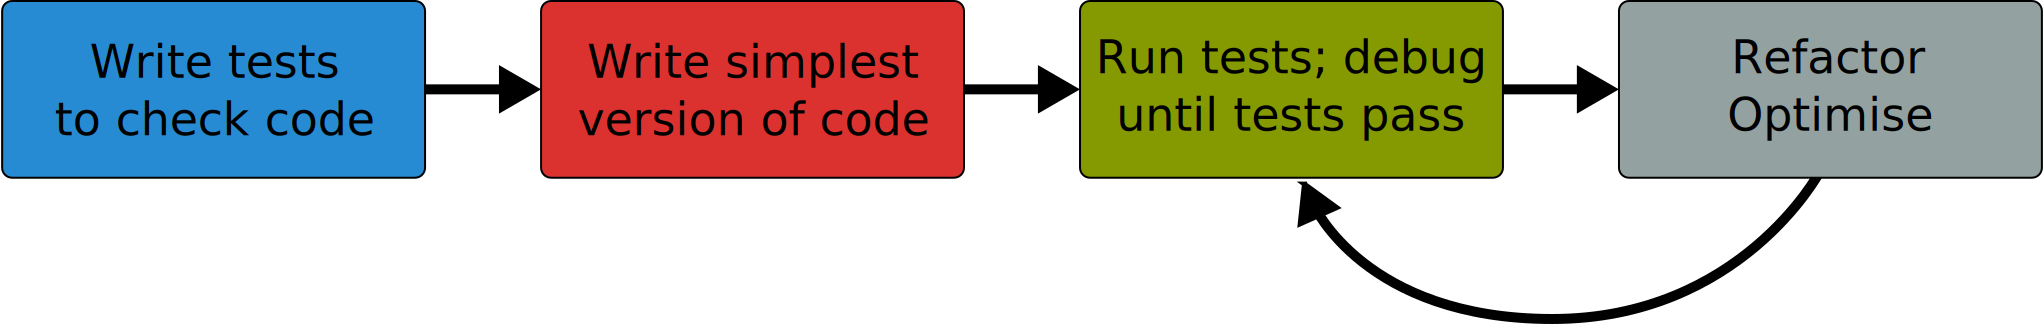
\includegraphics[width=1\textwidth]{images/testdriven.pdf}
\end{figure}

\begin{itemize}
  \item Define unit tests first!
  \item Develop one unit at a time!
\end{itemize}
  
\begin{itemize}
  \item more tomorrow
\end{itemize}

\end{frame}

% -------------------------------------

\end{document}
